\documentclass[14pt]{mmcs-article}
\usepackage[russian]{babel}
\usepackage{amsmath, amsthm, amsfonts, amssymb}
\usepackage{listings, listings-rust}

\graphicspath{{paper_images/}}
\newtheorem{theorem}{Теорема}
\newtheorem{notice}{Замечание}

% \newcounter{notice}[section]
% \newenvironment{notice}[1][]{\refstepcounter{notice}\par\medskip
%     \noindent \textbf{Замечание~\thenotice. #1} \rmfamily
% }
% {\medskip}

\newcounter{definition}[section]
\newenvironment{definition}[1][]{\refstepcounter{definition}\par\medskip
    \noindent \textbf{Определение~\thedefinition. #1} \rmfamily
}
{\medskip}

\begin{document}

\renewcommand{\mod}[1]{\textrm{mod}\ #1}

\section{Введение}

Многие современные алгоритмы помехоустойчивого кодирования используют двудольные графы с определёнными свойствами для коррекции ошибок при передаче данных через каналы с шумами. См., например, коды с малой плотностью проверок на чётность \cite{LDPC}. Из эмпирических данных следует, что для наиболее успешного кодирования следует использовать графы с максимальным обхватом.

Известны две основные группы методов построения таких двудольных графов: случайные, основанные на генерации начального графа случайным способом, например перебор возможных матриц \cite{bruteforce} и псевдослучайные пермутации матриц \cite{gallager}; и структурированные, основанные на построении графа с определённой, заранее известной структурой, например методы, использующие протографы \cite{protographs}.

% Написать про протографы

В настоящей статье предложен структурный метод построения двудольных графов с заданным, произвольно большим обхватом методом расширения метаграфов. Разработан алгоритм для выбора оптимальных весов для заданного метаграфов. Дана точная оценка максимального обхвата среди всех возможных расширений метаграфа на основе его структуры. Предложен алгоритм для итеративного подбора структуры метаграфа для построения расширения с заданным обхватом.

\section{Основные понятия и утверждения}

Приведём определения основных понятий используемых далее. Будем использовать определение двудольного графа на основе определения 7.1 данного в книге <<Дискретная Математика>> Я.М. Ерусалимского \cite{epyc_discrete_math}.

\begin{definition}
    \textsl{Двудольным графом} будем называть тройку $ G(V, E, f)$, такую, что:

\begin{itemize}
    \item $V = A \cup B$ и $A \cap B = \emptyset$ ;
    \item $f: E \rightarrow A \times B$ ;
\end{itemize}

Где $V$ ~-- множество вершин, разбитое на два непересекающихся подмножества $A$ и $B$.
$E$ ~-- множество дуг.
$f$ ~-- это отображение, определяющее то, с какими вершинами инцидентна дуга.

\end{definition}

\begin{definition}
    Последовательность дуг $\mu = (e_1, ..., e_d)$, такую что $e_i \neq e_{i+1}$ для любого $i < d$, будем называть путём с начальной вершиной $v_0$ и конечной вершиной $v_d$  на графе $G(V,E,f)$, если существует последовательность вершин $(v_0, ..., v_d)$ такая, что $\forall i = 1,...,d:$ $(v_i, v_{i+1}) = f(e_i)$ или $(v_{i+1}, v_i) = f(e_i)$. 

\end{definition}

\begin{definition}
    \textsl{Циклом} будем называть путь, у которого совпадают первая и последняя вершины.
\end{definition}

\begin{definition}
    \textsl{Обхватом графа} называют длину его минимального цикла.
\end{definition}

\begin{notice}
    Отметим, что обхват любого двудольного графа является чётным числом.
\end{notice}

\begin{notice}
    Известно, что на практике для кодирования эффективнее использовать графы с большим обхватом.
\end{notice}

\begin{definition}

С каждым путём $\mu$ свяжем характеристическую функцию $\chi_\mu(e)$:
\[
    \begin{array}{ll}
        \chi_{\mu}(e_1) = \left\{
            \begin{array}{ll}
            1,  & v_0 \in A;\\
            -1, & v_0 \in B. \\
            \end{array}
        \right. \\
        \chi_\mu(e_i) = -\chi_\mu(e_{i-1}) \forall i \in 2, ..., d\\
    \end{array}
\]

\end{definition}

\section{Метаграфы}

Далее будем рассматривать взвешенные двудольные графы на которых определена операция расширения, позволяющая строить графы со схожей структурой, но значительно большего размера, которые будем называть метаграфами. Метаграфы были ранее представлены в работах \cite{metagraphs} и \cite{metagraphs_2}

Дадим им формальное определение.

\begin{definition}
    Если $G(V,E,f)$ ~-- двудольный граф, то \textsl{Метаграфом} будем называть четвёрку $G'(V,E,f,w)$, где $w: E \to \mathbb{Z}$ ~-- отображения, задающее веса дуг.
\end{definition}

На рисунке \ref{image:2} представлен метаграф $G_1$ с тремя вершинами и четырьмя дугами.

\begin{figure}[H]
    \centering
    \begin{picture}(150,200)
        \put(75,165){\thicklines{\circle*{5}}}
        \put(70,170){$c_1$}
    
        \put(35,35){\thicklines{\circle*{5}}}
        \put(30,20){$i_1$}
    
        \put(115,35){\thicklines{\circle*{5}}}
        \put(110,20){$i_2$}
    
        \bezier{300}(75,165)(10,100)(35,35)
        \put(5,100){$+1$}

        \bezier{300}(75,165)(56,100)(35,35)
        \put(56,80){$0$}
    
        \bezier{300}(75,165)(140,100)(115,35)
        \put(125,100){$-1$}

        \bezier{300}(75,165)(94,100)(115,35)
        \put(87,80){$0$}
    \end{picture}
    \caption{ Метаграф с весами дуг +1, 0, 0, -1.. }
    \label{image:2}
\end{figure}

\begin{definition}
    Пусть $r \in \mathbb{N}$, тогда $r$-расширением метаграфа $G'(V,E,f,w)$ назовём граф $G^{(r)}(V^{(r)}, E^{(r)}, f^{(r)})$ построенный следующим образом: для каждой вершины $v \in V$ ставится в соответствие множество вершин $\{ v^{(1)}, ..., v^{(r)} \}$; для каждой дуги $e \in E$ ставится в соответствие множество дуг $\{ e^{(1)}, ..., e^{(r)} \}$, при этом если $f(e) = (a, b)$, тогда $f^{(r)}(e^{(i)}) = (a^{(i)}, b^{(i + w(e) (\mod{r}))})$ $\forall i = 1,...,r$.
\end{definition}

\begin{notice}
    Множества вершин и дуг расширения устроены следующим образом:
    \[
        V^{(r)} = \bigcup_{v \in V} \{ v^{(1)}, ..., v^{(r)} \};\;\;\;
        E^{(r)} = \bigcup_{e \in E} \{ e^{(1)}, ..., e^{(r)} \}.
    \]
\end{notice}


На рисунке. \ref{image:3} изображён граф, полученный 4-расширением метаграфа $G_1$, изображённого на рисунке \ref{image:2}.

\begin{figure}[H]
    \centering
    \begin{picture}(450,200)
        \put(75,165){\thicklines{\circle*{5}}}
        \put(70,170){$c_1$}
        \put(35,35){\thicklines{\circle*{5}}}
        \put(30,20){$i_1$}
        \put(115,35){\thicklines{\circle*{5}}}
        \put(110,20){$i_2$}

        \bezier{300}(75,165)(56,100)(35,35)
        \bezier{300}(75,165)(94,100)(115,35)
        \bezier{300}(75,165)(130,100)(135,35)
        \bezier{300}(175,165)(120,100)(115,35)

        \put(175,165){\thicklines{\circle*{5}}}
        \put(170,170){$c_1$}
        \put(135,35){\thicklines{\circle*{5}}}
        \put(130,20){$i_1$}
        \put(215,35){\thicklines{\circle*{5}}}
        \put(210,20){$i_2$}

        \bezier{300}(175,165)(156,100)(135,35)
        \bezier{300}(175,165)(194,100)(215,35)
        \bezier{300}(175,165)(230,100)(235,35)
        \bezier{300}(275,165)(220,100)(215,35)


        \put(275,165){\thicklines{\circle*{5}}}
        \put(270,170){$c_1$}
        \put(235,35){\thicklines{\circle*{5}}}
        \put(230,20){$i_1$}
        \put(315,35){\thicklines{\circle*{5}}}
        \put(310,20){$i_2$}

        \bezier{300}(275,165)(256,100)(235,35)
        \bezier{300}(275,165)(294,100)(315,35)
        \bezier{300}(275,165)(330,100)(335,35)
        \bezier{300}(375,165)(320,100)(315,35)


        \put(375,165){\thicklines{\circle*{5}}}
        \put(370,170){$c_1$}
        \put(335,35){\thicklines{\circle*{5}}}
        \put(330,20){$i_1$}
        \put(415,35){\thicklines{\circle*{5}}}
        \put(410,20){$i_2$}

        \bezier{300}(375,165)(356,100)(335,35)
        \bezier{300}(375,165)(394,100)(415,35)

        \bezier{700}(75,165)(245,100)(415,35)
        \bezier{700}(375,165)(205,100)(35,35)
    \end{picture}
    \caption{ Метаграф с весами дуг +1, 0, 0, -1.. }
    \label{image:3}
\end{figure}

\begin{theorem}[О начальных вершинах путей]
    Пусть $\eta = (e_1, \dots, e_d)$ ~-- путь с начальной вершиной $v$ на метаграфе $G$, тогда на графе $G^{(r)}$ существуют $r$ попарно не пересекающихся путей $\mu_1 \dots \mu_r$ с начальными вершинами $v^{(1)}, ..., v^{(r)}$, таких что для каждого пути $\mu'=(e_1',\dots,e_d') \in\{\mu_1,\dots,\mu_r\}$ справедливо, что для всех $j\in[1;d]_N$ $e_{j}' \in T^{(r)}(e_j)$.
\end{theorem}

\begin{proof}
    Доказательство этого утверждения практически дословно повторяет доказательство теоремы 1 в \cite{skorohodov_reachability_problem}.
\end{proof}

\begin{definition}
    Будем говорить, что пути $\eta$ на метаграфе $G$ соответствуют пути $\mu_i$ на графе $G^{(r)}$ и наоборот.
\end{definition}

\begin{notice}
    Из того, что некоторый путь на метаграфе $G$ является циклом не следует, что соответствующие ему пути на $G^{(r)}$ являются циклами. Рассмотрим эту ситуацию на следующем примере.
\end{notice}

\textbf{Пример 1.}

Рассмотрим граф на рисунке \ref{metagraph_3_expansion}. Путь $(e_1, e_2)$ является циклом на метаграфе, однако ни один из соответствующих ему путей $\mu_1 = (e^{(1)}_1, e^{(1)}_2)$, $\mu_2 = (e^{(2)}_1, e^{(2)}_2)$, $\mu_3 = (e^{(3)}_1, e^{(3)}_2)$  на 3-расширении не является циклом. При этом следует отметить, что склейка этих трёх путей порождает цикл $\mu = (e^{(1)}_1, e^{(1)}_2, e^{(2)}_1, e^{(2)}_2, e^{(3)}_1, e^{(3)}_2)$ длины 6. Заметим, что циклу $\mu$ соответствует цикл $(e_1, e_2, e_1, e_2, e_1, e_2)$ на метаграфе.

\begin{figure}[H]
    \centering
    \begin{picture}(255,200)
        \put(0,165){$a.$}

        \put(35,165){\thicklines{\circle*{5}}}
        \put(30,170){$A$}
        \put(35,35){\thicklines{\circle*{5}}}
        \put(30,20){$B$}
    
        \bezier{300}(35,165)(10,100)(35,35)
        \put(0,100){$e_1$}
        \bezier{300}(35,165)(60,100)(35,35)
        \put(56,100){$e_ 2$}



        \put(110,165){$b.$}

        \put(145,165){\thicklines{\circle*{5}}}
        \put(140,170){$A^{(1)}$}
        \put(145,35){\thicklines{\circle*{5}}}
        \put(140,20){$B^{(1)}$}

        \thicklines
        \bezier{300}(145,165)(145,100)(145,35)
        \put(125,130){$e_0^{(1)}$}

        \bezier{300}(145,165)(165,100)(185,35)
        \put(147,85){$e_1^{(1)}$}
        \thinlines

        \put(185,165){\thicklines{\circle*{5}}}
        \put(180,170){$A^{(2)}$}
        \put(185,35){\thicklines{\circle*{5}}}
        \put(180,20){$B^{(2)}$}

        \bezier{300}(185,165)(185,100)(185,35)
        \put(165,130){$e_0^{(2)}$}
        
        \bezier{300}(185,165)(205,100)(225,35)
        \put(187,85){$e_1^{(2)}$}

        \put(225,165){\thicklines{\circle*{5}}}
        \put(220,170){$A^{(3)}$}
        \put(225,35){\thicklines{\circle*{5}}}
        \put(220,20){$B^{(3)}$}

        \bezier{300}(225,165)(225,100)(225,35)
        \put(205,130){$e_0^{(3)}$}

        \bezier{300}(225,165)(232,50)(145,35)
        \put(190,45){$e_1^{(3)}$}
    \end{picture}
    \caption{ a. Метаграф. b. 3-расширение метаграфа. }
    \label{metagraph_3_expansion}
\end{figure}

\begin{definition}
    Пусть $G(V, E, f, w)$ ~-- метаграф.

Характеристикой пути $\eta = (e_1, ..., e_d)$ будем называть

\[
    \chi(\eta) = \sum_{i = 1}^d \chi_{\eta}(e_i) w(e_i).
\]

Ясно, что имеет место следующее утверждение:

\begin{theorem} \label{glued_paths}
    Пусть $G$ ~--- метаграф, $\mu = (e_1, \dots, e_d)$ и $\eta = (u_1, \dots, u_k)$ ~--- пути на $G$ и пусть $\xi = (e_1, \dots, e_d, u_1, \dots, u_k)$ является путём на $G$; пусть $\mu' = (e_d, \dots, e_1)$ получен из $\mu$ инвертированием.  Тогда имеют места следующие соотношения:

    1. $ \chi(\xi) = \chi(\mu) + \chi(\eta)$,

    2. $ \chi(\mu') = -\chi(\mu)$.
\end{theorem}

\end{definition}

\begin{theorem}[О конечных вершинах путей]

Пусть  $\eta = (e_1, ..., e_d)$ ~-- путь на метаграфе $G$, его первая вершина ~-- $x$, а последняя вершина ~-- $y$. И пусть $\mu' = (e'_1, ..., e'_d)$ один из соответствующих ему путей на расширенном графе.

Тогда если у $\mu'$ начальная вершина $x^{(i)}$, то его последняя вершина ~-- $y^{(i + \chi(\eta)\mod{r})}$.

\end{theorem}

\begin{proof}

Доказательство проведём по индукции по длине пути $|\eta| = d$.

Пусть $d = 1$, тогда путь состоит их одной дуги $e_1$.

Если $x \in A$, тогда вершина $x^{(i)}$ инцидентна дуге $e_1'$, для которой $f^{(r)}(e_1') = (x^{(i)}, y^{(i + w(e_1) (\mod{r}))})$ то есть, конечной вершиной пути $\mu_i$ является $y^{(i + w(e_1) (\mod{r}))} = y^{(i + \chi(\eta) (\mod{r}))}$.

Если $x \in B$, тогда вершина $x^{(i)}$ инцидентна дуге $e_1'$, для которой $f^{(r)}(e_1') = (y^{(i - w(e_1) (\mod{r}))}, x^{(i)})$ то есть, конечной вершиной пути $\mu_i$ является $y^{(i - w(e_1) (\mod{r}))} = y^{(i + \chi(\eta) (\mod{r}))}$.

Пусть условия теоремы выполняются для всякого $d < n$, тогда рассмотрим случай $d = n$.

Рассмотрим путь $\eta' = (e_1, ..., e_{d - 1})$. Обозначим его последнюю вершину $x$. Тогда по предположению индукции последние вершины соответствующих ему путей на метаграфе ~-- это $x^{(i + \chi(\eta')(\mod{r}))}$.

Если $x \in A$, тогда вершина $x^{(i + \chi(\eta')(\mod{r}))}$ инцидентна дуге \\ $f^{(r)}(e_d^{(i + \chi(\eta')(\mod{r}))}) = (x^{(i + \chi(\eta')(\mod{r}))}, y^{(i + \chi(\eta') + w(e_d) (\mod{r}))})$ и конечная \\ вершина пути $\mu_i$ ~-- $y^{(i + \chi(\eta') + w(e_d) (\mod{r}))} = y^{(i + \chi(\mu) (\mod{r}))}$.

Если $x \in B$, тогда вершина $x^{(i + \chi(\eta')(\mod{r}))}$ инцидентна дуге \\ $f^{(r)}(e_d^{(i + \chi(\eta') - w(e_d) (\mod{r}))}) = (y^{(i + \chi(\eta') - w(e_d) (\mod{r}))}, x^{(i)})$ и конечная вершина пути $\mu_i$ ~-- $y^{(i + \chi(\eta') - w(e_d) (\mod{r}))} = y^{(i + \chi(\mu) (\mod{r}))}$.

\end{proof}

Важными следствиями из Теоремы 2 являются две следующих теоремы.

\begin{theorem}[О циклах]

Пусть $\eta$ ~-- цикл на метаграфе. Тогда соответствующие ему пути на расширенном графе являются циклами тогда и только тогда, когда $\chi(\eta) = 0 (\mod{r})$.

\end{theorem}

\begin{theorem}[О <<крыльях>> цикла]

Пусть $\eta = (e_1, ..., e_d)$ и $\mu = (\epsilon_1, ..., \epsilon_{\delta})$ ~-- различные пути на метаграфе с начальной вершиной $a$, конечной вершиной $b$ и $\chi(\eta) = \chi(\mu) (\mod{r})$. Тогда путь на расширении, соответствующий склейке этих путей $\gamma = (e_1, \dots, e_d, \epsilon_{\delta}, \dots, \epsilon_1)$, является циклом.

\end{theorem}

\section{Построение графов с заданным обхватом}

Пусть $G(V, E, f, w)$ ~-- метаграф $w(e_i) = x_i \forall i = 0..|E|$.

Для циклов $\eta$ на метаграфе $G$, длина которых меньше $2l$, рассмотрим не равенства вида $\chi(\eta) \neq 0$.

Систему, содержащую все такие не равенств представим в виде (1).

\begin{equation}
    \centering
    \left\{
        \begin{array}{ll}
            a_{1,1} x_1 + ... + a_{1,e} x_e + b &\neq 0 ; \\
            ...\\
            a_{l,1} x_1 + ... + a_{n,e} x_e + b &\neq 0 .\\
        \end{array}
    \right..
    \label{eqs:example}
\end{equation}

Пусть $G$ ~-- некоторый метаграф. Тогда справедлива следующая теорема.

\begin{theorem}

Для $G$ существует расширение с обхватом большим $2l$  тогда и только тогда, когда система не равенств (1) для графа $G$ совместна.

\end{theorem}

\begin{proof}

При построении системы (1) исчерпываются все циклы, следовательно существование решения системы (1) эквивалентно существованию расширения с обхватом большим $2l$.

\end{proof}

Для построения системы вида \ref{eqs:example} для заданного метаграфа $G$ можно воспользоваться следующим алгоритмом.

\textbf{Алгоритм 1.}

Пусть $G(A \cup B, E, f, w)$ ~-- метаграф причём $w(e_i) = x_i \forall i = 0..|E|$.

Алгоритм основан на заполнении множества меток для вершин метаграфа. Каждая метка представляет собой четвёрку $(g, v, ch, p)$, где $g$ ~-- длина пути $\mu$ пройденного от начальной до помечаемой вершины, далее $g$ будем называть поколением метки; $v$ ~-- вершина, которая помечена этой меткой; $ch \in \mathbb{Z}$ ~-- характеристика метки, обозначает характеристику пути $\mu$; $p \in V \cup \{ nil \}$ ~-- дуга, на основе которой была сгенерирована метка, при обработке предыдущего поколения меток, где $nil \not\in V $ ~-- специальное значение, зарезервированное для исходной метки.

Для каждой вершины $a \in A$:

\begin{itemize}
    \item Добавим метку $(0, a, 0, nil)$ в пустое множество всех меток
    \item В цикле по поколениям $g$ от $1$ до $l / 2$:
    \begin{itemize}
        \item Для всех меток вида $(g - 1, v, ch, p)$:
        \item
            Для каждой дуги $e \not= p$ инцидентной вершине $v$,
            формируем метку $(g, v', ch', e)$, где $ch' = ch + (-1)^{g} w(e)$, $v'$ ~-- вершина отличная от $v$, инцидентная $e$.
            Добавляем эту метку ко множеству всех меток.
    \end{itemize}
    \item Добавляем в систему, все не равенства вида, $ch_1 \neq \ch_2$ для всех пар меток с совпадающими вершинами и поколениями.
\end{itemize}

\begin{notice}
    В алгоритме 1  рассматриваются циклы, состоящие из двух путей одинаковой длины, проходящих через одну вершину, то есть будут найдены только циклы состоящие из двух <<крыльев>> одинаковой длины, однако любой цикл на метаграфе представим в таком виде, следовательно будут найдены все циклы.
\end{notice}

\textbf{Пример.}

На рисунке \ref{neq_system_graph} изображён метаграф с четырьмя дугами $e_1, e_2, e_3, e_4$. Веса которых ~-- неизвестные, $x_1, x_2, x_3, x_4$ соответственно.

Выполним алгоритм 2 с заданным обхватом 6 с данным метаграфом в качестве входного параметра. Множество меток, сгенерированное в ходе работы данного алгоритма показано в таблице \ref{cycle_search_table_neq}. По этому множеству меток затем была построена система не равенств (2), её решение даёт набор весов, которые, будучи подставленными в метаграф позволят построить r-расширение с обхватом 6.

\begin{figure}[H]
    \centering
    \begin{picture}(150,200)
        \put(75,165){\thicklines{\circle*{5}}}
        \put(70,170){$v_1$}
    
        \put(35,35){\thicklines{\circle*{5}}}
        \put(30,20){$v_2$}
    
        \put(115,35){\thicklines{\circle*{5}}}
        \put(110,20){$v_3$}
    
        \bezier{300}(75,165)(10,100)(35,35)
        \put(5,100){$x_1$}

        \bezier{300}(75,165)(56,100)(35,35)
        \put(56,80){$x_2$}
    
        \bezier{300}(75,165)(140,100)(115,35)
        \put(125,100){$x_3$}

        \bezier{300}(75,165)(94,100)(115,35)
        \put(87,80){$x_4$}
    \end{picture}
    \caption{ Метаграф, дуги которого имеют веса, заданные переменными $x_1, x_2, x_3, x_4$. }
    \label{neq_system_graph}
\end{figure}

\begin{table}[H]
    \centering
    \begin{tabular}{ | c | c | c | }
        \hline
        $g = 0$            & $g = 1$               & $g = 2$                   \\ \hline
        $(0, v_1, 0, nil)$ & $(1, v_2,  x_1, e_1)$ & $(2, v_1,  x_1 - x_2, b)$ \\ \hline
                           & $(1, v_2,  x_2, e_2)$ & $(2, v_1,  x_2 - x_1, a)$ \\ \hline
                           & $(1, v_3,  x_3, e_3)$ & $(2, v_1,  x_3 - x_4, e)$ \\ \hline
                           & $(1, v_3,  x_4, e_4)$ & $(2, v_1,  x_4 - x_3, d)$ \\ \hline
    \end{tabular}
    \caption{ Множество меток, сгенерированное в процессе работы алгоритма построения системы уравнений. }
    \label{cycle_search_table_neq}
\end{table}

\begin{equation}
    \centering
    \left\{
        \begin{array}{ll}
            x_1 - x_2 &\neq 0             ; \\
            x_3 - x_4 &\neq 0             ; \\
            2 x_1 - 2 x_2 &\neq 0         ; \\
            2 x_3 - 2 x_4 &\neq 0         ; \\
            x_1 - x_2 - x_3 + x_4 &\neq 0 ; \\
            x_1 - x_2 + x_3 - x_4 &\neq 0 . \\
        \end{array}
        \label{eqs:cycle_search_neqs}
    \right.
\end{equation}

\section{Решение систем не равенств}

Поиск минимального решения для систем не равенств вида (\ref{eqs:example}), представленных в прошлой главе представляется вычислительно трудной задачей. Она предполагает перебор всех возможных решений с выбором минимального. Однако некоторое решение можно найти, воспользовавшись следующим алгоритмом.

\textbf{Алгоритм 2.}

\begin{enumerate}
    \item $e$ ~-- количество неизвестных в системе не равенств.
    \item Если в системе содержится не равенство вида $0 \neq 0$, то система не имеет решений, алгоритм завершается, сообщая, что решений нет.
    \item Найдём все не равенства вида $a x_e + b \neq 0$. Обозначим множество таких не равенств $I$.
    \item Выберем число $v$ такое, что $v \neq -b/a \forall a x_e + b \in I$, если $I = \varnothing$, то положим $v = 0$. Такое число можно найти, так как не равенств конечное количество. В результате этой замены не возникнет не равенства вида $0 \neq 0$ по условию выбора $v$.
    \item Заменим во всех не равенствах $x_e$ на $v$ и добавим в решение элемент $x_e = v$.
    \item Если $e = 1$ ~-- завершим работу алгоритма.
    \item Положим $e = e - 1$ переменной и вернёмся на шаг 3.
\end{enumerate}

\textbf{Пример.}

Положим $x_1 = 0$, подставим в систему не равенств, получим:

\begin{equation}
    \centering
    \left\{
        \begin{array}{ll}
            - x_2 &\neq 0            ; \\
            x_3 - x_4 &\neq 0        ; \\
            - 2 x_2 &\neq 0          ; \\
            - 2 x_4 &\neq 0          ; \\
            - x_2 - x_3 + x_4 &\neq 0; \\
            - x_2 + x_3 - x_4 &\neq 0. \\
        \end{array}
    \right..
    \label{eqs:cycle_search_neqs}
\end{equation}

Значение $x_2$ не может быть равно $0$, т.к. в таком случае нарушается не равенство $- x_2 \neq 0$. Положим $x_2 = 1$, подставим в систему не равенств, получим:

\begin{equation}
    \centering
    \left\{
        \begin{array}{ll}
            - 1 &\neq 0             ; \\
            x_3 - x_4 &\neq 0       ; \\
            - 2 &\neq 0             ; \\
            - 2 x_4 &\neq 0         ; \\
            - 1 - x_3 + x_4 &\neq 0 ; \\
            - 1 + x_3 - x_4 &\neq 0 . \\
        \end{array}
    \right..
    \label{eqs:cycle_search_neqs}
\end{equation}

Положим $x_3 = 0$, подставим в систему не равенств, получим:

\begin{equation}
    \centering
    \left\{
        \begin{array}{ll}
            - 1 &\neq 0       ; \\
            - x_4 &\neq 0     ; \\
            - 2 &\neq 0       ; \\
            - 2 x_4 &\neq 0   ; \\
            - 1 + x_4 &\neq 0 ; \\
            - 1 - x_4 &\neq 0 . \\
        \end{array}
    \right..
    \label{eqs:cycle_search_neqs}
\end{equation}

Значение $x_4$ не может принимать значения $0, 1, -1$, т.к. в таком случае нарушаются не равенства. Положим $x_4 = 2$, подставим в систему не равенств, получим:

\begin{equation}
    \centering
    \left\{
        \begin{array}{ll}
            - 1 &\neq 0   ; \\
            - 2 &\neq 0   ; \\
            - 2 &\neq 0   ; \\
            - 4 &\neq 0   ; \\
            1 &\neq 0     ; \\
            - 3 &\neq 0   . \\
        \end{array}
    \right..
    \label{eqs:cycle_search_neqs}
\end{equation}

Полученные не равенства показывают, что $r$ не может принимать значения $1, 2, 3, 4$, следовательно минимально допустимое значение $r$ ~-- $5$. 5-расширение метаграфа с весами, полученными в ходе решения системы не равенств, изображено на рисунке \ref{neq_system_res}. Заметим, что действительно обхват этого графа равен 6, один из циклов-шестёрок выделен жирным.

\begin{figure}[H]
    \centering
    \begin{picture}(380,200)
        \put(50,165){\thicklines{\circle*{5}}}
        \put(35,35){\thicklines{\circle*{5}}}
        \put(65,35){\thicklines{\circle*{5}}}
    
        \bezier{300}(50,165)(42,100)(35,35)
        \bezier{300}(50,165)(57,100)(65,35)


        \put(120,165){\thicklines{\circle*{5}}}
        \put(105,35){\thicklines{\circle*{5}}}
        \put(135,35){\thicklines{\circle*{5}}}

        \bezier{300}(120,165)(127,100)(135,35)
        \bezier{300}(120,165)(197,100)(275,35)

        \put(190,165){\thicklines{\circle*{5}}}
        \put(175,35){\thicklines{\circle*{5}}}
        \put(205,35){\thicklines{\circle*{5}}}

        \bezier{300}(190,165)(217,100)(245,35)
        \bezier{300}(190,165)(267,100)(345,35)

        \put(260,165){\thicklines{\circle*{5}}}
        \put(245,35){\thicklines{\circle*{5}}}
        \put(275,35){\thicklines{\circle*{5}}}

        \bezier{300}(260,165)(252,100)(245,35)
        \bezier{300}(260,165)(267,100)(275,35)
        \bezier{300}(260,165)(287,100)(315,35)
        \bezier{600}(260,165)(172,50)(65,35)

        \put(330,165){\thicklines{\circle*{5}}}
        \put(315,35){\thicklines{\circle*{5}}}
        \put(345,35){\thicklines{\circle*{5}}}

        \bezier{300}(330,165)(322,100)(315,35)
        \bezier{300}(330,165)(337,100)(345,35)
        \bezier{600}(330,165)(182,150)(35,35)
        \bezier{600}(330,165)(242,50)(135,35)

        \thicklines
        \bezier{300}(50,165)(77,100)(105,35)
        \bezier{300}(120,165)(112,100)(105,35)
        \bezier{300}(120,165)(147,100)(175,35)
        \bezier{300}(190,165)(182,100)(175,35)
        \bezier{300}(190,165)(197,100)(205,35)
        \bezier{300}(50,165)(127,100)(205,35)
    \end{picture}
    \caption{ Расширение метаграфа с весами дуг, полученными решением системы не равенств. }
    \label{neq_system_res}
\end{figure}

\begin{notice}
    Результатом работы алгоритма поиска решения системы не равенств не обязательно будет минимальное решение.
\end{notice}

\section{Выбор структуры метаграфа}

В предыдущих разделах был получен способ находить веса, позволяющие построить r-расширение метаграфа с заданным обхватом. Однако не было предложена способа выбирать структуру самого метаграфа так, чтобы была возможность отыскать такие веса т.е. чтобы результатом алгоритма 2 была непротиворичивая система не равенств.

\begin{definition}
    Под обхватом метаграфа с неопределёнными весами будем понимать максимальный из обхватов, который можно получить у r-расширения этого метаграфа в результате подбора весов.
\end{definition}

\begin{notice}
    Последовательно запуская алгоритм 2 с одним и тем же входным метаграфом с неопределёнными весами и различным требуемым обхватом расширения, можно определить его обхват ~-- это максимальное число, для которого алгоритм завершается успешно.
\end{notice}

Изучим метаграфы, построенные на основе полных двудольных графов. 

\begin{definition}
    Будем называть двудольный граф $G(V,E,f)$, такой что $V = A \cup B, A \cap B = \emptyset$ полным, если для каждой пары вершин $a \in A, b \in B$ существует единственная дуга $e$, такая что $f(e) = (a, b)$.
\end{definition}

Пример одного из таких графов изображён на рисунке \ref{full_graph_3_by_9}. 

\begin{figure}[H]
    \centering
    \begin{picture}(300,200)
        \put(65,165){\thicklines{\circle*{5}}}
        \put(155,165){\thicklines{\circle*{5}}}
        \put(245,165){\thicklines{\circle*{5}}}

        \put(35,35){\thicklines{\circle*{5}}}
        \put(65,35){\thicklines{\circle*{5}}}
        \put(95,35){\thicklines{\circle*{5}}}

        \bezier{500}(35,35)(35,35)(65,165)
        \bezier{500}(65,35)(65,35)(65,165)
        \bezier{500}(95,35)(95,35)(65,165)
        \bezier{500}(35,35)(35,35)(155,165)
        \bezier{500}(65,35)(65,35)(155,165)
        \bezier{500}(95,35)(95,35)(155,165)
        \bezier{500}(35,35)(35,35)(245,165)
        \bezier{500}(65,35)(65,35)(245,165)
        \bezier{500}(95,35)(95,35)(245,165)

        \put(125,35){\thicklines{\circle*{5}}}
        \put(155,35){\thicklines{\circle*{5}}}
        \put(185,35){\thicklines{\circle*{5}}}

        \bezier{500}(125,35)(125,35)(65,165)
        \bezier{500}(155,35)(155,35)(65,165)
        \bezier{500}(185,35)(185,35)(65,165)
        \bezier{500}(125,35)(125,35)(155,165)
        \bezier{500}(155,35)(155,35)(155,165)
        \bezier{500}(185,35)(185,35)(155,165)
        \bezier{500}(125,35)(125,35)(245,165)
        \bezier{500}(155,35)(155,35)(245,165)
        \bezier{500}(185,35)(185,35)(245,165)

        \put(215,35){\thicklines{\circle*{5}}}
        \put(245,35){\thicklines{\circle*{5}}}
        \put(275,35){\thicklines{\circle*{5}}}

        \bezier{500}(215,35)(215,35)(65,165)
        \bezier{500}(245,35)(245,35)(65,165)
        \bezier{500}(275,35)(275,35)(65,165)
        \bezier{500}(215,35)(215,35)(155,165)
        \bezier{500}(245,35)(245,35)(155,165)
        \bezier{500}(275,35)(275,35)(155,165)
        \bezier{500}(215,35)(215,35)(245,165)
        \bezier{500}(245,35)(245,35)(245,165)
        \bezier{500}(275,35)(275,35)(245,165)
    \end{picture}
    \caption{ Пример полного двудольного графа с тремя информационными и девятью проверочными вершинами. }
    \label{full_graph_3_by_9}
\end{figure}


\begin{notice}
    Отметим, что во всяком полном метаграфе, в котором есть хотя бы две информационные и три проверочные вершины возникнет цикл длины 12. Рассмотрим метаграф на рисунке \ref{full_graph_2_by_3}. Рассмотрим цикл $\mu = (e_1, e_4, e_5, e_2, e_3, e_6, e_4, e_1, e_2, e_5, e_6, e_3)$. Его характеристика равна $x_1 - x_4 + x_5 - x_2 + x_3 - x_6 + x_4 - x_1 + x_2 - x_5 + x_6 - e_3 = 0$. Следовательно, этот путь будет являться циклом на r-расширении этого метаграфа. 
\end{notice}

Таким образом для построения графов с обхватом большим 12 необходимо использовать неполные метаграфы.

\begin{figure}[H]
    \centering
    \begin{picture}(200,200)
        \put(65,165){\thicklines{\circle*{5}}}
        \put(155,165){\thicklines{\circle*{5}}}

        \put(35,35){\thicklines{\circle*{5}}}
        \put(110,35){\thicklines{\circle*{5}}}
        \put(185,35){\thicklines{\circle*{5}}}

        \bezier{500}(35,35)(35,35)(65,165)
        \put(40,140){$e_1$}
        \bezier{500}(110,35)(110,35)(65,165)
        \put(65,120){$e_2$}
        \bezier{500}(185,35)(185,35)(65,165)
        \put(85,150){$e_3$}

        \bezier{500}(35,35)(35,35)(155,165)
        \put(125,150){$e_4$}
        \bezier{500}(110,35)(110,35)(155,165)
        \put(145,120){$e_5$}
        \bezier{500}(185,35)(185,35)(155,165)
        \put(165,140){$e_6$}
    \end{picture}
    \caption{ Пример полносвязаного метаграфа с двумя информационными и тремя проверочными вершинами. }
    \label{full_graph_2_by_3}
\end{figure}

\textbf{Определение.}

Пусть $G$ ~--- граф, такой что 

\begin{theorem}

    Пусть $G(V, E, f, w)$ ~-- метаграф, веса дуг которого ~-- неизвестные; $\mu$ ~--- цикл на метаграфе $G$; $a$, $b$ ~--- две возможно совпадающих вершины на цикле $\mu$; $\eta$ ~--- путь с начально вершиной $a$ и конечной вершиной $b$, такой что первая и последняя дуги этого пути не совпадают с дугами цикла $\mu$ смежными с вершинами $a$ и $b$; тогда максимальный обхват графа, полученного расширение этого метаграфа будет не больше $2(|\mu| + |\eta|)$.

\end{theorem}

\begin{proof}

    Обозначим пути, полученные прохождением по $\mu$ и $\eta$ в обратную сторону соответственно $\mu'$ и $\eta'$.

    Обозначим последовательность дуг, полученный склейкой $\nu = (\eta, \mu, \eta', \mu')$. В этой последовательности нет двух совпадающих дуг идущих подряд, т.к. начальные и конечные дуги пути $\eta$ не совпадают с дугами цикла $\mu$ смежными с вершинами $a$ и $b$, следовательно эта склейка является циклом на $G$.

    Вычислим длину $\nu$: $|\nu| = 2(|\mu| + |\eta|)$.

    Применяя теорему \ref{glued_paths} вычислим характеристику $\nu$: $\chi(\nu) = \chi(\eta) + \chi(\mu) + \chi(\eta') + \chi(\mu') = \chi(\eta) + \chi(\mu) - \chi(\eta) - \chi(\mu) = 0$.

    Следовательно $\mu$ ~-- цикл на всяком r-расширении $G$.

\end{proof}

\textbf{Теорема.}

Пусть $G'$ ~--- двудольный граф. Обозначим $\theta = \min\limits_{H \in \Phi(G')} \{ |H| \}$. Тогда существует набор весов дуг графа $G'$ такой, что для полученного метаграфа существовало расширение с обхватом равным $2 \theta$.

\begin{proof}

Рассмотрим такие циклы на метаграфе, которые соответствуют циклам длины меньшей $2 \theta$ на некоторых расширениях, но существуют расширения, на которых таким циклам соответствуют пути, не являющиеся циклами.

Следовательно, можно используя Алгоритм 1 подобрать веса и $r$ такие что всем таким циклам будут соответствовать не циклы на расширениях. Таким образом можно ограничиться рассмотрением только тех расширений, на которых подобные циклы уже разорваны,  и рассматривать такие циклы на метаграфе, которым соответствуют циклы на всех расширениях. Обхваты всех таких расширений будут одинаковыми. Поэтому рассмотрим самый короткий из таких циклов.

Если циклу на метаграфе соответствуют циклы на всех расширениях, значит его характеристика обращается в $0$ вне зависимости от выбранных весов. Значит такой цикл проходит каждую свою дугу равное количество раз в противоположные стороны. 

Путь не может проходить одну и ту же дугу дважды подряд, значит его структура распадается на несколько циклов, которые склеиваются в вершине степени не меньше трёх. Эта структура соответствует циклу с ручкой или циклу с ручкой объединённому с дополнительными путями. Таким образом длина такого цикла будет не меньше, чем удвоенная длина цикла с ручкой. По предыдущей теореме, его длина не больше, чем удвоенная длина цикла с ручкой. Получаем, что длина такого цикла равна $2 \theta$.

\end{proof}

\textbf{Алгоритм 3.}

Для построения графа обхват которого не меньше произвольного заданного числа, можно использовать следующий алгоритм:

\begin{itemize}
    \item Построить $G_0$ ~-- полный граф, его обхват ~-- 4.
    \item Построить $G_1$ с использованием алгоритма 2, используя граф $G_0$ в качестве структуры метаграфа. Обхват $G_1$ больше или равен 6.
    \item Повторяем предыдущий пункт до тех пор, получая графы со всё большим обхватом, пока не получим граф с требуемым обхватом.  
\end{itemize}

\textbf{Пример.}

Применим данный алгоритм для получения (2,3)-регулярного двудольного графа с обхватом 14.

Построим (2,3)-регулярный полный метаграф. Он состоит из двух проверочных и трёх информационных вершин и имеет обхват 4. Такой граф изображён на рисунке \ref{full_graph_2_by_3}.

На рисунке \ref{be_not_afraid} изображён двудольный граф с обхватом 8, полученный из полного метаграфа с помощью алгоритма 2, с последующим 3-расширением. Об содержит 6 проверочных и 9 информационных вершин. Проверочные вершины расположены на внутренней окружности, а информационные на внешней. Вершины сгруппированы в соответствие с соответствующими им вершинами на метаграфе.

\begin{figure}[H]
    \centering
    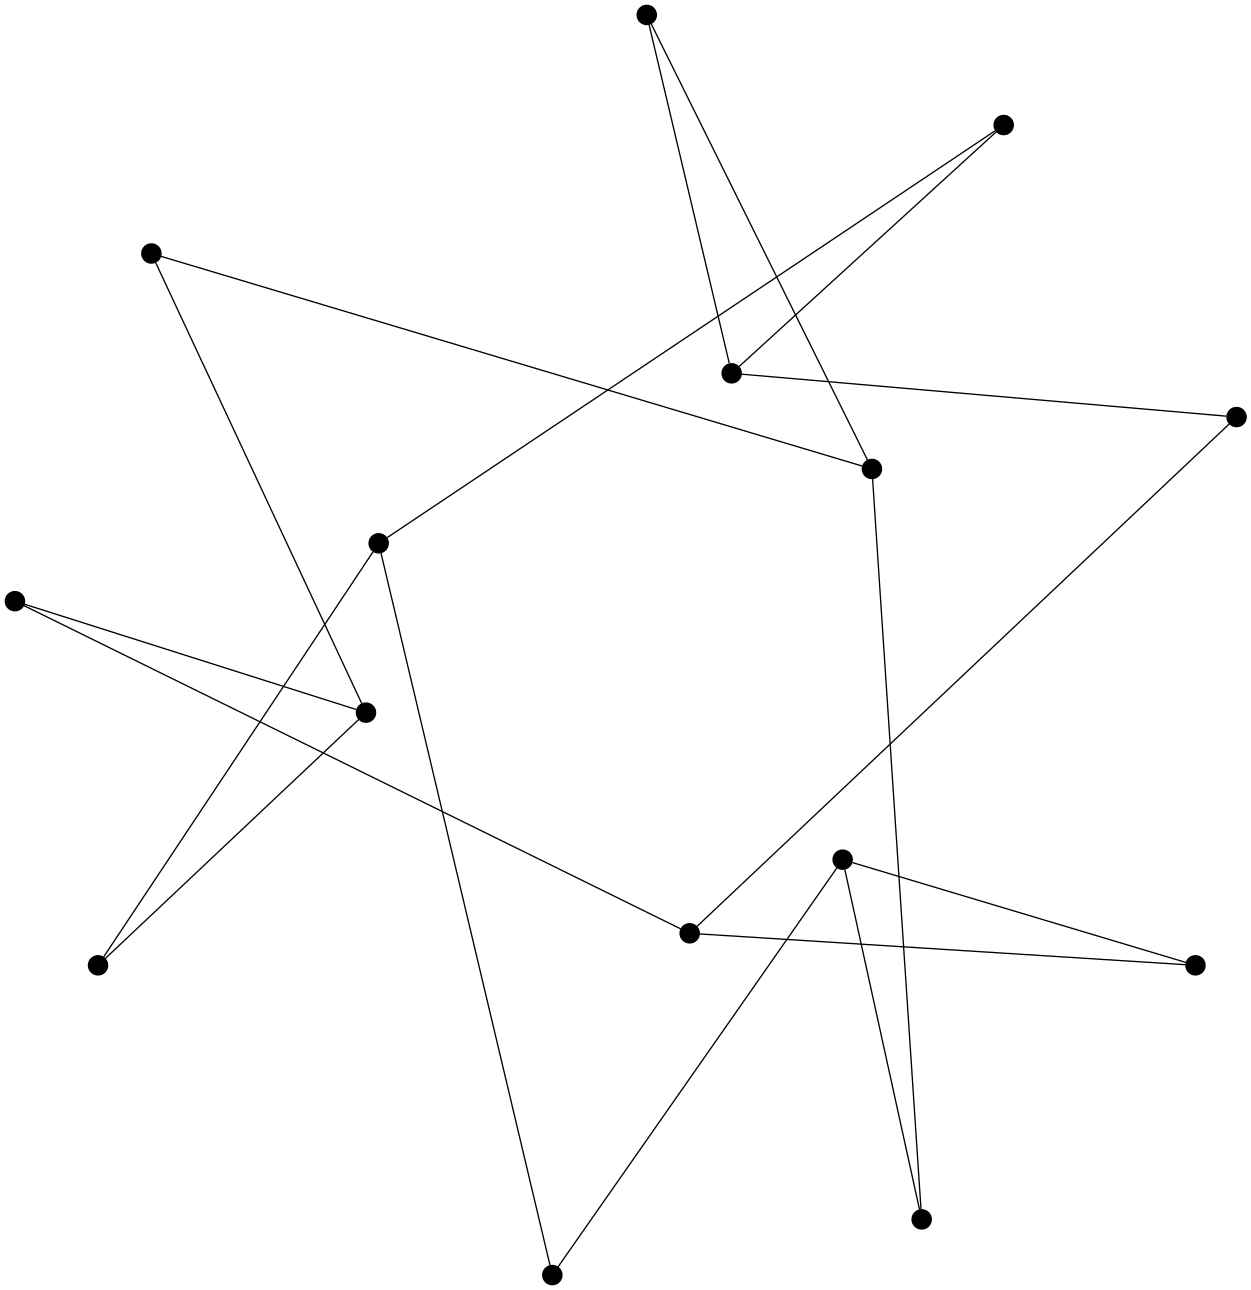
\includegraphics[scale=0.2]{graph_2.png}
    \caption{ (2,3)-регулярный двудольный граф с обхватом 8. }
    \label{be_not_afraid}
\end{figure}

На рисунке \ref{be_not_afraid_2} изображён двудольный граф с обхватом 14, полученный из метаграфа, построенного на основе двудольного графа с обхватом 6 из предыдущего пункта с помощью алгоритма 2, с последующим 7-расширением. Он содержит 42 проверочных и 63 информационных вершины.

\begin{figure}[H]
    \centering
    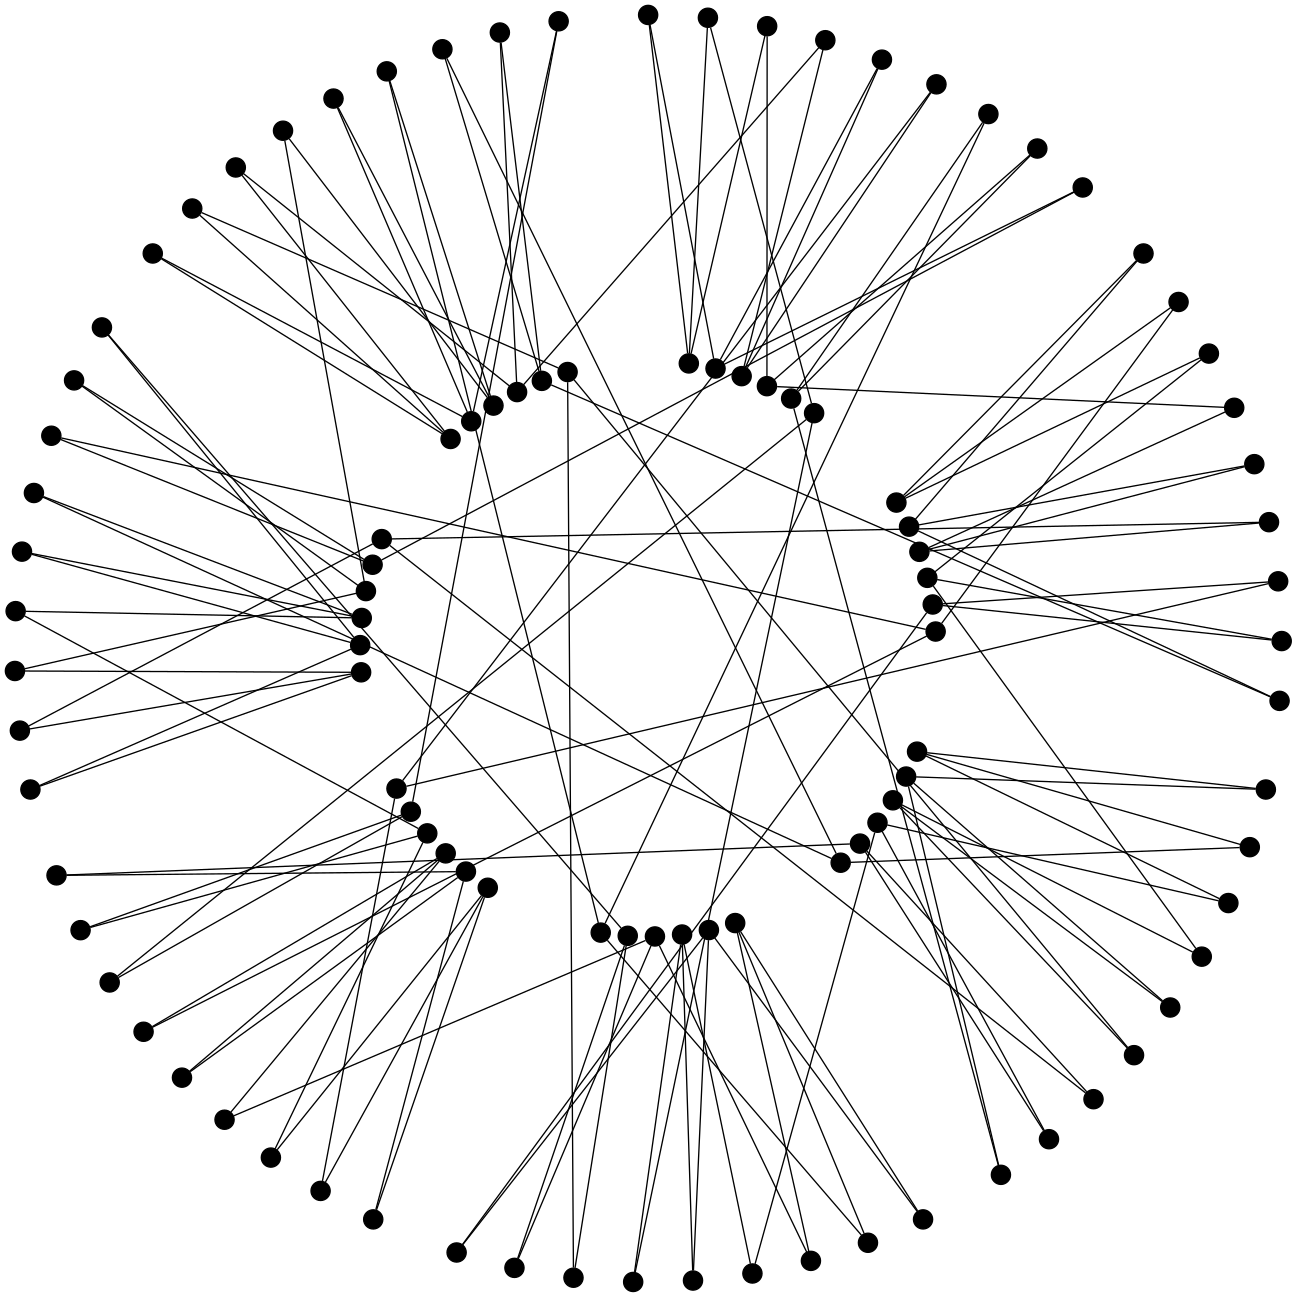
\includegraphics[scale=0.2]{graph_3.png}
    \caption{ (2,3)-регулярный двудольный граф с обхватом 14. }
    \label{be_not_afraid_2}
\end{figure}


\begin{notice}
    Граф с большим обхватом 14 несколькими способами: например построив сначала граф с обхватом 6, а по нему ~-- с обхватом 14, или сначала построить граф с обхватом 12 и по нему с обхватом 14. Доказательство наличия оптимального варианта построения, которое бы породило граф минимального размера, выходит за рамки данной работы, однако мы приведём практическое наблюдение, что лучше минимизировать количество шагов, а при равном количестве шагов, минимизировать размеры более ранних этапов.
\end{notice}

%=======================
\newpage

\addcontentsline{toc}{section}{Литература}
\renewcommand{\refname}{\centering \textbf{Литература}}

\begin{thebibliography}{0}

\bibitem{zemor}
G. Zémor, On Expander Codes, IEEE Trans. on Information theory, IT-47
No 2, (2001) pp. 835–837.
  
\bibitem{johnson}
S.\,J. Johnson,
Introducing Low-Density Parity-Check Codes.
~-- University of Newcastle, Australia, 2006.

\bibitem{gallager}
R.\,G. Gallager,
Low-density parity-check codes
~-- IRE Transactions on Information Theory, 1962.

\bibitem{bruteforce}
Гурский С.\,С., Могилевская Н.\,С.
Задача генерации проверочных матриц ldpc-кодов.
~-- Ростов н/Д : Материалы конференции СИТО, 2021.

\bibitem{protographs}
J. Thorpe,
Low-density parity-check (LDPC) codes constructed from protographs.
~-- JPL, IPN Progress Rep., Aug. 2003, vol. 42–154.

\bibitem{metagraphs}
Арутюнов О.\,В.
Построение (m, n)-регулярных двудольных графов с наибольшим обхватом методом увеличения метаграфов.
~-- Ростов н/Д : Материалы конференции СИТО, 2021.

\bibitem{metagraphs_2}
Арутюнов О.\,В.
Построение двудольных графов с заданным обхватом методом расширения метаграфов.
~-- Ростов н/Д : Материалы конференции СИТО, 2022.

\bibitem{epyc_discrete_math}
Я.М. Ерусалимский,
Дискретная Математика: теория, задачи и приложение. 3-е издание.
~-- Москва, <<Вузовская книга>>, 2000г.

\bibitem{skorohodov_reachability_problem}
Skorokhodov V.A. Generalization of the Reachability Problem on Directed Graphs
~-- Mathematics and Statistics, Vol. 8, No. 6, pp. 699 - 704, 2020. DOI: 10.13189/ms.2020.080610

\end{thebibliography}

\end{document}